%%
% The BIThesis Template for Bachelor Graduation Thesis
%
% 北京理工大学毕业设计(论文) —— 使用 XeLaTeX 编译
%
% Copyright 2021 BITNP
%
% This work may be distributed and/or modified under the
% conditions of the LaTeX Project Public License, either version 1.3
% of this license or (at your option) any later version.
% The latest version of this license is in
%   http://www.latex-project.org/lppl.txt
% and version 1.3 or later is part of all distributions of LaTeX
% version 2005/12/01 or later.
%
% This work has the LPPL maintenance status `maintained'.
%
% The Current Maintainer of this work is Feng Kaiyu.
%
% Compile with: xelatex -> biber -> xelatex -> xelatex

% 章节支持、单面打印:ctexbook
\documentclass[bachelor,footskip=24pt]{bitbook}
% 如果想要修改样式,但无法找到样式在哪里定义:请参考 https://bithesis.bitnp.net/Guide/4-Others/Troubleshooting.html#%E6%83%B3%E8%A6%81%E4%BF%AE%E6%94%B9%E9%83%A8%E5%88%86%E6%A0%B7%E5%BC%8F-%E4%BD%86%E6%98%AF%E6%89%BE%E4%B8%8D%E5%88%B0%E6%A0%B7%E5%BC%8F%E5%9C%A8%E5%93%AA%E9%87%8C%E5%AE%9A%E4%B9%89

% 另一个临时的“修改页眉文字”的解决方法(非常不优雅,只作为临时措施)。
% 请注释掉以下 20 行内容使用。
% % 从原有主题继承自定义主题
% \fancypagestyle{BIThesisCustom}[BIThesis]{
%   % 定义页眉、页码
%   \fancyhead[C]{\zihao{4}\ziju{0.08}\songti{北京理工大学本科生毕业设计(论文)覆盖}}
% }
% % 设置章节格式
% \ctexset{chapter={
%     pagestyle = BIThesisCustom,
%   }
% }
% % 前置页面(原创性声明、中英文摘要、目录等)
% \renewcommand{\frontmatter}{
%   \pagenumbering{Roman}
%   \pagestyle{BIThesisCustom}
% }
% % 正文页面
% \renewcommand{\mainmatter}{
%   \pagenumbering{arabic}
%   \pagestyle{BIThesisCustom}
% }
% ------------------------------------------------------------------

% 使用 listings 宏包进行代码块使用,并使用了预定义的样式,
% 你也可以选用自己的喜欢的其他宏包,如 minted;
% 然而由于 minted 依赖 Python 的 Pygments 库作为外部依赖,因此出于模板的建议性考虑,我们没有提供 minted 进行代码块书写的示例。
% 但是,我们仍旧非常建议你使用 minted。
\usepackage{listings}
\usepackage{hyperref}


% 参考文献引用文件位于 misc/ref.bib
\addbibresource{misc/ref.bib}

% 在这里填写你的论文中英文题目
\newcommand{\thesisTitle}{北京理工大学本科生毕业设计(论文)题目}
\newcommand{\thesisTitleEN}{The Subject of Undergraduate Graduation Project (Thesis) of Beijing Institute of Technology}

% 在这里填写你的相关信息
\newcommand{\deptName}{计算机学院}
\newcommand{\majorName}{计算机科学与技术}
\newcommand{\yourName}{张国安}
\newcommand{\yourStudentID}{1120181447}
\newcommand{\mentorName}{陆慧梅}
% 如果你的毕设为校外毕设,请将下面这一行语句解除注释(删除第一个百分号字符)并在第二组花括号中填写你的校外毕设导师名字
% \newcommand{\externalMentorName}{左偏树}

% 文档开始
\begin{document}

% 标题页面:如无特殊需要,本部分无需改动
%%
% The BIThesis Template for Bachelor Graduation Thesis
%
% 北京理工大学毕业设计(论文)封面页 —— 使用 XeLaTeX 编译
%
% Copyright 2020-2021 BITNP
%
% This work may be distributed and/or modified under the
% conditions of the LaTeX Project Public License, either version 1.3
% of this license or (at your option) any later version.
% The latest version of this license is in
%   http://www.latex-project.org/lppl.txt
% and version 1.3 or later is part of all distributions of LaTeX
% version 2005/12/01 or later.
%
% This work has the LPPL maintenance status `maintained'.
%
% The Current Maintainer of this work is Feng Kaiyu.
%
% 封面
%
% 如无特殊需要,本页面无需更改

% Underline new command for student information
% Usage: \dunderline[<offset>]{<line_thickness>}
\newcommand\dunderline[3][-1pt]{{%
  \setbox0=\hbox{#3}
  \ooalign{\copy0\cr\rule[\dimexpr#1-#2\relax]{\wd0}{#2}}}}

% Cover Page
\begin{titlepage}
  \makeatletter
  \@ifundefined{externalMentorName}{
    % 校内毕设封面顶部间距
    \vspace*{19mm}
  }{
    % 校外毕设封面顶部间距
    \vspace*{13mm}
  }
  \centering

  
\includegraphics[width=9.87cm]{images/header.png}

  \vspace*{-3mm}

  \zihao{-0}\textbf{\ziju{0.12}\songti{本科生毕业设计(论文)}}

  \vspace{16mm}

  \zihao{2}\textbf{\xihei\thesisTitle}

  \vspace{3mm}

  \begin{spacing}{1.2}
    \zihao{3}\selectfont{\textbf{\thesisTitleEN}}
  \end{spacing}

  \vspace{15mm}

  \flushleft

  \makeatletter
  \@ifundefined{externalMentorName}{
    % 生成校内毕设封面字段
    \makeatother
    \begin{spacing}{1.8}
      \hspace{27mm}\songti\zihao{3}\selectfont{学\hspace{11mm}院:\dunderline[-10pt]{1pt}{\makebox[78mm][c]{\deptName}}}

      \hspace{27mm}\songti\zihao{3}\selectfont{专\hspace{11mm}业:\dunderline[-10pt]{1pt}{\makebox[78mm][c]{\majorName}}}

      \hspace{27mm}\songti\zihao{3}\selectfont{学生姓名:\dunderline[-10pt]{1pt}{\makebox[78mm][c]{\yourName}}}

      \hspace{27mm}\songti\zihao{3}\selectfont{学\hspace{11mm}号:\dunderline[-10pt]{1pt}{\makebox[78mm][c]{\yourStudentID}}}

      \hspace{27mm}\songti\zihao{3}\selectfont{指导教师:\dunderline[-10pt]{1pt}{\makebox[78mm][c]{\mentorName}}}
    \end{spacing}
  }{
    % 生成校外毕设封面字段
    \makeatother
    \begin{spacing}{1.8}
      \hspace{19.4mm}\songti\zihao{3}\selectfont{学\hspace{19.6mm}院\hspace{3mm}:\dunderline[-10pt]{1pt}{\makebox[77.4mm][c]{\deptName}}}

      \hspace{19.4mm}\songti\zihao{3}\selectfont{专\hspace{19.6mm}业\hspace{3mm}:\dunderline[-10pt]{1pt}{\makebox[77.4mm][c]{\majorName}}}

      \hspace{19.4mm}\songti\zihao{3}\selectfont{学\hspace{2.8mm}生\hspace{2.8mm}姓\hspace{2.8mm}名\hspace{3mm}:\dunderline[-10pt]{1pt}{\makebox[77.4mm][c]{\yourName}}}

      \hspace{19.4mm}\songti\zihao{3}\selectfont{学\hspace{19.6mm}号\hspace{3mm}:\dunderline[-10pt]{1pt}{\makebox[77.4mm][c]{\yourStudentID}}}

      \hspace{19.4mm}\songti\zihao{3}\selectfont{指\hspace{2.8mm}导\hspace{2.8mm}教\hspace{2.8mm}师\hspace{3mm}:\dunderline[-10pt]{1pt}{\makebox[77.4mm][c]{\mentorName}}}

      \hspace{19.4mm}\songti\zihao{3}\selectfont{校外指导教师:\dunderline[-10pt]{1pt}{\makebox[77.4mm][c]{\externalMentorName}}}
    \end{spacing}
  }

  \vspace*{\fill}
  \centering
  \zihao{3}\ziju{0.5}\songti{\today}
\end{titlepage}


% 前置页面定义
\frontmatter
% 原创性声明:如无特殊需要,本部分无需改动
% 更改为 PDF 页面插入,如需要添加内容,可考虑先用 Word 制作再覆盖 misc/1_originality.pdf

\includepdf{misc/1_originality.pdf}
\newpage
%%%
% The BIThesis Template for Bachelor Graduation Thesis
%
% 北京理工大学毕业设计(论文)原创性声明页 —— 使用 XeLaTeX 编译
%
% Copyright 2020-2021 BITNP
%
% This work may be distributed and/or modified under the
% conditions of the LaTeX Project Public License, either version 1.3
% of this license or (at your option) any later version.
% The latest version of this license is in
%   http://www.latex-project.org/lppl.txt
% and version 1.3 or later is part of all distributions of LaTeX
% version 2005/12/01 or later.
%
% This work has the LPPL maintenance status `maintained'.
%
% The Current Maintainer of this work is Feng Kaiyu.
%
% 如无特殊需要,本页面无需更改

% 原创性声明页无页码页面格式
\fancypagestyle{originality}{
  % 页眉高度
  \setlength{\headheight}{20pt}

  % 页眉和页脚(页码)的格式设定
  \fancyhf{}
  \fancyhead[C]{\zihao{4}\ziju{0.08}\songti{北京理工大学本科生毕业设计(论文)}}

  % 页眉分割线稍微粗一些
  \renewcommand{\headrulewidth}{0.6pt}
}

\pagestyle{originality}
\topskip=0pt

% 圆形数字编号定义
\newcommand{\circled}[2][]{\tikz[baseline=(char.base)]
  {\node[shape = circle, draw, inner sep = 1pt]
  (char) {\phantom{\ifblank{#1}{#2}{#1}}};
  \node at (char.center) {\makebox[0pt][c]{#2}};}}
\robustify{\circled}

% 设置行间距
\setlength{\parskip}{0.4em}
\renewcommand{\baselinestretch}{1.41}

% 顶部空白
\vspace*{-6mm}

% 原创性声明部分
\begin{center}
  \heiti\zihao{2}\textbf{原创性声明}
\end{center}

% 本部分字号为小三
\zihao{-3}

本人郑重声明:所呈交的毕业设计(论文),是本人在指导老师的指导下独立进行研究所取得的成果。除文中已经注明引用的内容外,本文不包含任何其他个人或集体已经发表或撰写过的研究成果。对本文的研究做出重要贡献的个人和集体,均已在文中以明确方式标明。

特此申明。

\vspace{13mm}

\begin{flushright}
  本人签名:\hspace{40mm}日\hspace{2.5mm}期:\hspace{13mm}年\hspace{8mm}月\hspace{8mm}日
\end{flushright}

\vspace{17mm}

% 使用授权声明部分
\begin{center}
  \heiti\zihao{2}\textbf{关于使用授权的声明}
\end{center}

本人完全了解北京理工大学有关保管、使用毕业设计(论文)的规定,其中包括:\circled{1}学校有权保管、并向有关部门送交本毕业设计(论文)的原件与复印件;\circled{2}学校可以采用影印、缩印或其它复制手段复制并保存本毕业设计(论文);\circled{3}学校可允许本毕业设计(论文)被查阅或借阅;\circled{4}学校可以学术交流为目的,复制赠送和交换本毕业设计(论文);\circled{5}学校可以公布本毕业设计(论文)的全部或部分内容。

\vspace*{1mm}

\begin{flushright}
  \begin{spacing}{1.65}
    \zihao{-3}
    本人签名:\hspace{40mm}日\hspace{2.5mm}期:\hspace{13mm}年\hspace{8mm}月\hspace{8mm}日\\
    指导老师签名:\hspace{40mm}日\hspace{2.5mm}期:\hspace{13mm}年\hspace{8mm}月\hspace{8mm}日
  \end{spacing}
\end{flushright}

\newpage

% 摘要:在摘要相应的 TeX 文件处进行摘要部分的撰写
%%
% The BIThesis Template for Bachelor Graduation Thesis
%
% 北京理工大学毕业设计(论文)中英文摘要 —— 使用 XeLaTeX 编译
%
% Copyright 2020-2021 BITNP
%
% This work may be distributed and/or modified under the
% conditions of the LaTeX Project Public License, either version 1.3
% of this license or (at your option) any later version.
% The latest version of this license is in
%   http://www.latex-project.org/lppl.txt
% and version 1.3 or later is part of all distributions of LaTeX
% version 2005/12/01 or later.
%
% This work has the LPPL maintenance status `maintained'.
%
% The Current Maintainer of this work is Feng Kaiyu.

% 中英文摘要章节
\zihao{-4}
\vspace*{-11mm}

\begin{center}
  \heiti\zihao{-2}\textbf{\thesisTitle}
\end{center}

\vspace*{2mm}

{\let\clearpage\relax \chapter*{\textmd{摘~~~~要}}}
\addcontentsline{toc}{chapter}{摘~~~~要}
\setcounter{page}{1}

\vspace*{1mm}

\setstretch{1.53}
\setlength{\parskip}{0em}

% 中文摘要正文从这里开始
操作系统课程是计算机专业的重要专业基础课,
其对于培养学生的工程能力与设计能力有着很大的意义。
而操作系统实验部分更是课程的核心内容,
该部分可以让学生在实践中学习操作系统的算法、工程实现、设计思想。

代理内核是不具备独立I/O实现的操作系统内核,
它的提出了为了支持受到I/O限制的RISC-V CPU。
它的所依赖的I/O功能都代理给了宿主机上的操作系统。
它具有轻量、代码精简的优点。

本文是基于华中科技大学的代理内核操作系统实验的移植和改进。
本文从源代码层面,经济成本与学习成本方面,
分析了代理内核实验在教学过程中存在的优点与缺点。
对于其目前存在的经济成本高、环境搭建复杂等缺点,本文提出了实验改进的需求。
然后进行需求分析,并给出了移植到K210开发板上的解决方案。
最后本文给出了移植代理内核操作系统实验到K210开发板上的具体实现,
并编写了相关的实验指导书。完成了对代理内核操作系统实验的移植与改进。

\vspace{4ex}\noindent\textbf{\heiti 关键词:操作系统;内核;代理内核;实验改进;K210;移植}
\newpage

% 英文摘要章节
\vspace*{-2mm}

\begin{spacing}{0.95}
  \centering
  \heiti\zihao{3}\textbf{\thesisTitleEN}
\end{spacing}

\vspace*{17mm}

{\let\clearpage\relax \chapter*{
  \zihao{-3}\textmd{Abstract}\vskip -3bp}}
\addcontentsline{toc}{chapter}{Abstract}
\setcounter{page}{2}

\setstretch{1.53}
\setlength{\parskip}{0em}

% 英文摘要正文从这里开始
The operating system course is an important professional course for the students major in Computer Science,
It is of great significance to develop students' engineering ability and design ability.
The operating system experiment is the core content of the course,
This part allows students to learn the algorithm, 
engineering implementation and design idea of the operating system in practice.

The RISC-V Proxy Kernel is an operating system without independent I/O implementation.
It is designed to support tethered RISC-V implementations with limited I/O capability and thus handles I/O-related system calls by proxying them to a host computer.
It has the advantages of light weight and simplified code.

This paper is based on the transplantation and improvement of the Proxy Kernel operating system experiment of Huazhong University of Science and Technology.
From the perspective of source code, economic cost and learning cost,
we analyze the advantages and disadvantages of Proxy Kernel experiment in the teaching process.
This paper puts forward the disadvantages of high cost and complex experimental environment.
Then the requirements analysis is carried out, and the solution which transplanted PKE to K210 development board is given.
Finally, this paper gives the concrete implementation of the solution,
and then gives the tutorial of the experiment.

\vspace{3ex}\noindent\textbf{Key Words: Operating System;Proxy Kernel;Improvement;K210;Transplantation}
\newpage

% 目录:如无特殊需要,本部分无需改动
%%
% The BIThesis Template for Bachelor Graduation Thesis
%
% 北京理工大学毕业设计(论文)目录 —— 使用 XeLaTeX 编译
%
% Copyright 2020-2021 BITNP
%
% This work may be distributed and/or modified under the
% conditions of the LaTeX Project Public License, either version 1.3
% of this license or (at your option) any later version.
% The latest version of this license is in
%   http://www.latex-project.org/lppl.txt
% and version 1.3 or later is part of all distributions of LaTeX
% version 2005/12/01 or later.
%
% This work has the LPPL maintenance status `maintained'.
%
% The Current Maintainer of this work is Feng Kaiyu.
%
% 如无特殊需要,本页面无需更改

% 目录开始

% 调整目录行间距
\renewcommand{\baselinestretch}{1.35}
% 目录
\tableofcontents
\newpage


% 正文开始
\mainmatter
% 正文 22 磅的行距
\setlength{\parskip}{0em}
\renewcommand{\baselinestretch}{1.53}
% 修复脚注出现跨页的问题
\interfootnotelinepenalty=10000

% 第一章
%%
% The BIThesis Template for Bachelor Graduation Thesis
%
% 北京理工大学毕业设计(论文)第一章节 —— 使用 XeLaTeX 编译
%
% Copyright 2020-2021 BITNP
%
% This work may be distributed and/or modified under the
% conditions of the LaTeX Project Public License, either version 1.3
% of this license or (at your option) any later version.
% The latest version of this license is in
%   http://www.latex-project.org/lppl.txt
% and version 1.3 or later is part of all distributions of LaTeX
% version 2005/12/01 or later.
%
% This work has the LPPL maintenance status `maintained'.
%
% The Current Maintainer of this work is Feng Kaiyu.
%
% 第一章节

\chapter{背景}

\section{二级题目}
% 这里插入一个参考文献,仅作参考
正文……\cite{yuFeiJiZongTiDuoXueKeSheJiYouHuaDeXianZhuangYuFaZhanFangXiang2008}

\subsection{三级题目}

正文……\cite{Hajela2012Application}

\textcolor{blue}{正文部分:宋体、小四;正文行距:22磅;间距段前段后均为0行。阅后删除此段。}

\textcolor{blue}{图、表居中,图注标在图下方,表头标在表上方,宋体、五号、居中,1.25倍行距,间距段前段后均为0行,图表与上下文之间各空一行。阅后删除此段。}

\textcolor{blue}{\underline{\underline{图-示例:(阅后删除此段)}}}

\begin{figure}[htbp]
  \vspace{13pt} % 调整图片与上文的垂直距离
  \centering
  
\includegraphics[]{images/bit_logo.png}
  \caption{标题序号}\label{标题序号} % label 用来在文中索引
\end{figure}

\textcolor{blue}{\underline{\underline{表-示例:(阅后删除此段)}}}

\begin{table}[htbp]
  \linespread{1.5}
  \zihao{5}
  \centering
  \caption{统计表}\label{统计表}
  \begin{tabular}{*{5}{>{\centering\arraybackslash}p{2cm}}}
    \hline
    项目    & 产量    & 销量    & 产值   & 比重    \\ \hline
    手机    & 1000  & 10000 & 500  & 50\%  \\
    计算机   & 5500  & 5000  & 220  & 22\%  \\
    笔记本电脑 & 1100  & 1000  & 280  & 28\%  \\ \hline
    合计    & 17600 & 16000 & 1000 & 100\% \\ \hline
    \end{tabular}
\end{table}

\textcolor{blue}{公式标注应于该公式所在行的最右侧。对于较长的公式只可在符号处(+、-、*、/、$\leqslant$ $\geqslant$ 等)转行。在文中引用公式时,在标号前加“式”,如式(1-2)。阅后删除此
段。}

\textcolor{blue}{公式-示例:(阅后删除此段)}
% 公式上下不要空行,置于同一个段落下即可,否则上下距离会出现高度不一致的问题
\begin{equation}
    LRI=1\ ∕\ \sqrt{1+{\left(\frac{{\mu }_{R}}{{\mu }_{s}}\right)}^{2}{\left(\frac{{\delta }_{R}}{{\delta }_{s}}\right)}^{2}}
\end{equation}

\subsubsection{生僻字}

% 一个可能无法正常显示的生僻字
一个可能无法正常显示的生僻字: 彧。下文注释中,介绍了如何通过自定义字体来显示生僻字。

% 定义一个提供了生僻字的字体,注意要确保你的系统存在该字体
% \setCJKfamilyfont{custom-font}{Noto Serif CJK SC}

% 使用自己定义的字体
% 使用提供了相应字型的字体:\CJKfamily{custom-font}{彧}。


% 在这里添加第二章、第三章……TeX 文件的引用
 %%
% The BIThesis Template for Bachelor Graduation Thesis
%
% 北京理工大学毕业设计(论文)第二章节 —— 使用 XeLaTeX 编译
%
% Copyright 2020-2021 BITNP
%
% This work may be distributed and/or modified under the
% conditions of the LaTeX Project Public License, either version 1.3
% of this license or (at your option) any later version.
% The latest version of this license is in
%   http://www.latex-project.org/lppl.txt
% and version 1.3 or later is part of all distributions of LaTeX
% version 2005/12/01 or later.
%
% This work has the LPPL maintenance status `maintained'.
%
% The Current Maintainer of this work is Feng Kaiyu.
%%

\chapter{环境搭建}

\section{软件环境}

\subsection{编译工具链}
step1.访问sifive官网,下载riscv gcc toolchain

\href{https://www.sifive.com/software}{https://www.sifive.com/software}

step2.找到Prebuilt RISC-V GCC Toolchain。根据开发环境选择对应的版本。

\begin{figure}[htbp]
    \vspace{13pt} % 调整图片与上文的垂直距离
    \centering
    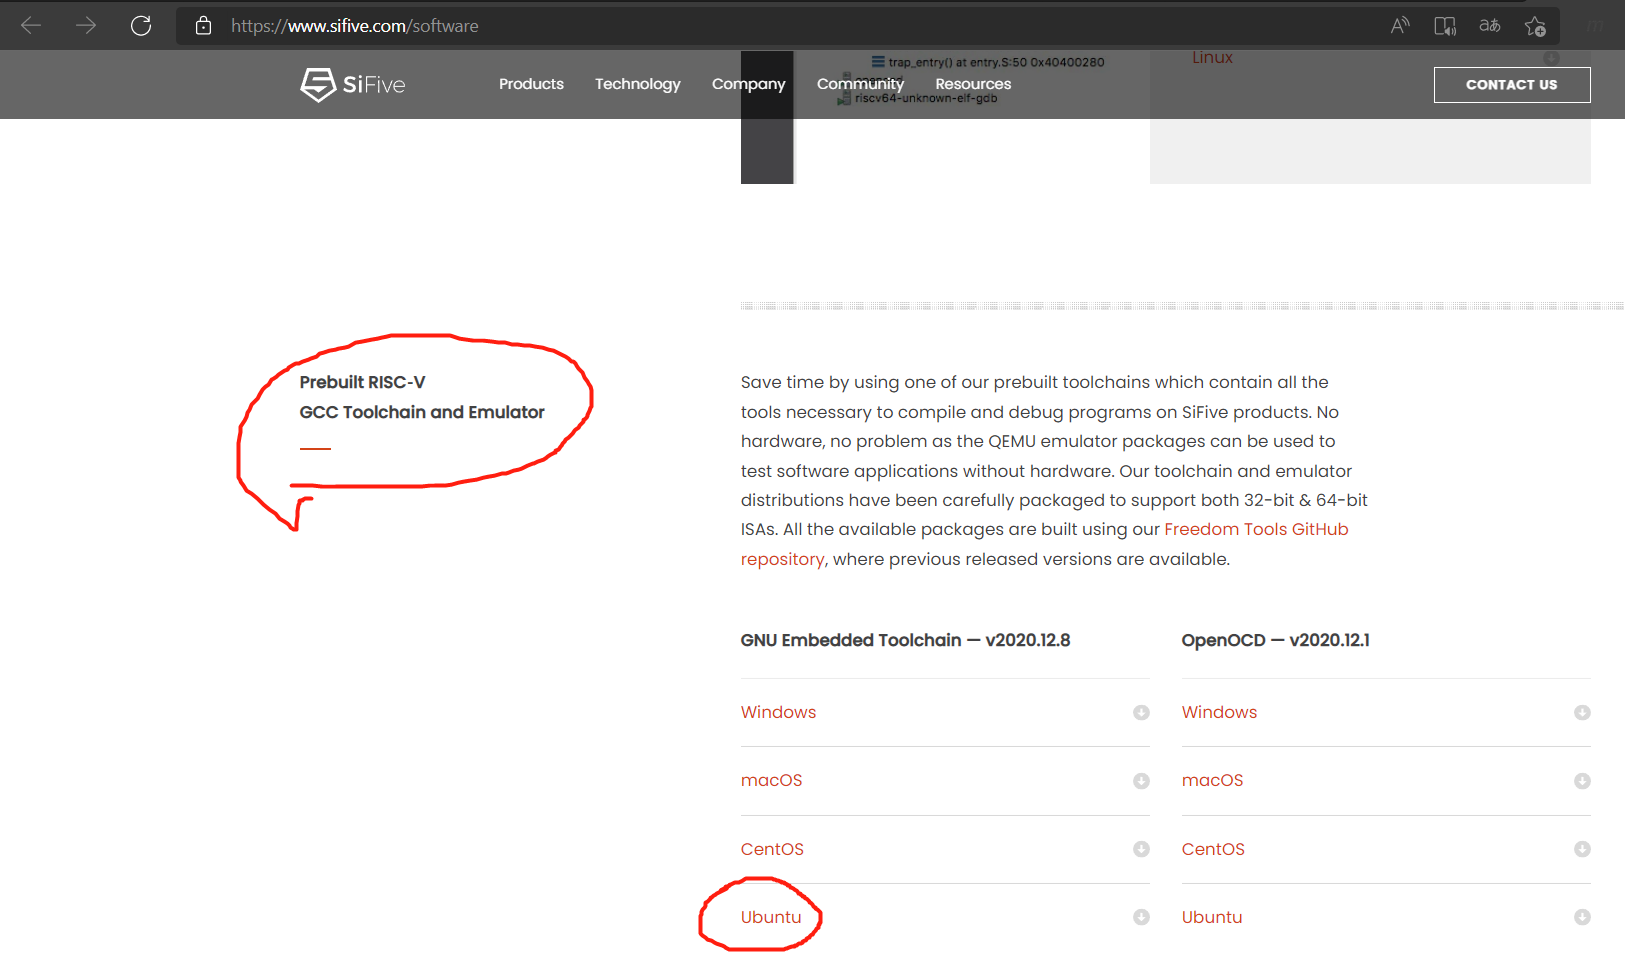
\includegraphics[width=0.8\textwidth]{images/toolchain.png}
    \caption{编译工具链列表}\label{编译工具链列表} % label 用来在文中索引
\end{figure}

step3.将下载好的tar.gz压缩包解压

\begin{lstlisting}[caption={解压命令}, label={lst:tar_command}]
    tar -zxvf $your_tar_gz
\end{lstlisting}

step4.配置环境变量。解压完成得到文件夹,进入文件夹里的bin目录,打开terminal,输入pwd获得当前路径。
复制获得的路径。将复制到的路径加入系统的PATH环境变量。

\begin{lstlisting}[caption={修改环境变量}, label={lst:change_env}]
    vim /etc/profile
    #添加以下两行到文件末尾
    export RISCV=$your_path
    export PATH=$PATH:$RISCV
\end{lstlisting}

\begin{figure}[htbp]
    \vspace{13pt} % 调整图片与上文的垂直距离
    \centering
    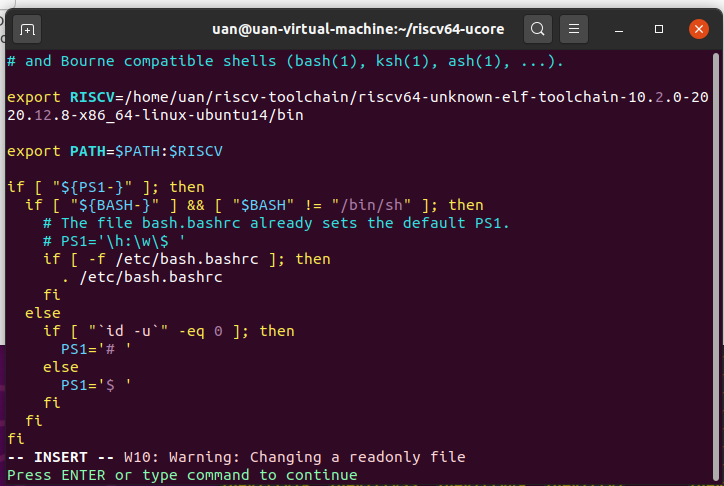
\includegraphics[width=0.8\textwidth]{images/env_path.png}
    \caption{配置环境变量}\label{配置环境变量} % label 用来在文中索引
\end{figure}

step5.加载环境变量文件

\begin{lstlisting}[caption={加载环境变量文件}, label={lst:load_env_profile}]
    source /etc/profile
\end{lstlisting}

step6.验证编译环境

在终端输入 riscv64-unknown-elf-gcc -v,如果出现以下内容,则编译环境配置成功。

\begin{lstlisting}[caption={验证编译环境}, label={lst:check_env}]
    Using built-in specs.
    ....
    gcc version 10.2.0 (SiFive GCC-Metal 10.2.0-2020.12.8) 
\end{lstlisting}

\subsection{代码准备}

step1.下载riscv64-pke-k210的代码库并查看所有分支

\begin{lstlisting}[caption={下载代码库}, label={lst:download_code}]
    git clone git@github.com:BITzga/riscv64-pke-k210.git
    git branch -a
\end{lstlisting}

step2.根据开发需求选择分支。

如下所示,k210前缀的代码分支是根据k210环境移植完成的代码。而其他普通分支则是PKE原先的代码。此时,根据开发需求使用git checkout命令选择分支即可。

\begin{lstlisting}[caption={分支列表}, label={lst:branch_list}]
    remotes/origin/k210/lab1_1_syscall
    remotes/origin/k210/lab1_2_exception
    remotes/origin/k210/lab1_3_irq
    remotes/origin/k210/lab2_1_pagetable
    remotes/origin/k210/lab2_2_allocatepage
    remotes/origin/k210/lab2_3_pagefault
    remotes/origin/k210/lab3_1_fork
    remotes/origin/k210/lab3_2_yield
    remotes/origin/k210/lab3_3_rrsched
    remotes/origin/lab1_1_syscall
    remotes/origin/lab1_2_exception
    remotes/origin/lab1_3_irq
    remotes/origin/lab2_1_pagetable
    remotes/origin/lab2_2_allocatepage
    remotes/origin/lab2_3_pagefault
    remotes/origin/lab3_1_fork
    remotes/origin/lab3_2_yield
    remotes/origin/lab3_3_rrsched
    remotes/origin/master
\end{lstlisting}


\subsection{编辑器、IDE选择}

\subsection{K210环境}

RustSBI-K210支持

Python3环境

烧录工具

串口调试环境



\section{硬件环境}

\subsection{K210硬件要求}

% 
\chapter{编译流程及内核启动流程改造}

\section{二级题目}
% 这里插入一个参考文献,仅作参考
正文……\cite{yuFeiJiZongTiDuoXueKeSheJiYouHuaDeXianZhuangYuFaZhanFangXiang2008}

\subsection{三级题目}

正文……\cite{Hajela2012Application}



% 结论:在结论相应的 TeX 文件处进行结论部分的撰写
%%
% The BIThesis Template for Bachelor Graduation Thesis
%
% 北京理工大学毕业设计(论文)结论 —— 使用 XeLaTeX 编译
%
% Copyright 2020-2021 BITNP
%
% This work may be distributed and/or modified under the
% conditions of the LaTeX Project Public License, either version 1.3
% of this license or (at your option) any later version.
% The latest version of this license is in
%   http://www.latex-project.org/lppl.txt
% and version 1.3 or later is part of all distributions of LaTeX
% version 2005/12/01 or later.
%
% This work has the LPPL maintenance status `maintained'.
%
% The Current Maintainer of this work is Feng Kaiyu.
%
% Compile with: xelatex -> biber -> xelatex -> xelatex

\unnumchapter{结~~~~论}
\renewcommand{\thechapter}{结论}

\ctexset{
  section/number = \arabic{section}
}

% 结论部分尽量不使用 \subsection 二级标题,只使用 \section 一级标题

% 这里插入一个参考文献,仅作参考
本文结论……。\cite{李成智2004飞行之梦}

\textcolor{blue}{结论作为毕业设计(论文)正文的最后部分单独排写,但不加章号。结论是对整个论文主要结果的总结。在结论中应明确指出本研究的创新点,对其应用前景和社会、经济价值等加以预测和评价,并指出今后进一步在本研究方向进行研究工作的展望与设想。结论部分的撰写应简明扼要,突出创新性。阅后删除此段。}

\textcolor{blue}{结论正文样式与文章正文相同:宋体、小四;行距:22 磅;间距段前段后均为 0 行。阅后删除此段。}

% 参考文献:如无特殊需要,参考文献相应的 TeX 文件无需改动,添加参考文献请使用 BibTeX 的格式
%   添加至 misc/ref.bib 中,并在正文的相应位置使用 \cite{xxx} 的格式引用参考文献
%%
% The BIThesis Template for Bachelor Graduation Thesis
%
% 北京理工大学毕业设计(论文)参考文献 —— 使用 XeLaTeX 编译
%
% Copyright 2020-2021 BITNP
%
% This work may be distributed and/or modified under the
% conditions of the LaTeX Project Public License, either version 1.3
% of this license or (at your option) any later version.
% The latest version of this license is in
%   http://www.latex-project.org/lppl.txt
% and version 1.3 or later is part of all distributions of LaTeX
% version 2005/12/01 or later.
%
% This work has the LPPL maintenance status `maintained'.
%
% The Current Maintainer of this work is Feng Kaiyu.
%
% Compile with: xelatex -> biber -> xelatex -> xelatex
%
% 如无特殊需要,本页面无需更改

% 参考文献开始
\unnumchapter{参考文献}
\renewcommand{\thechapter}{参考文献}

% 设置参考文献字号为 5 号
\renewcommand*{\bibfont}{\zihao{5}}
% 设置参考文献各个项目之间的垂直距离为 0
\setlength{\bibitemsep}{0ex}
\setlength{\bibnamesep}{0ex}
\setlength{\bibinitsep}{0ex}
% 设置单倍行距
\renewcommand{\baselinestretch}{1.2}
% 设置参考文献顺序标签 `[1]` 与文献内容 `作者. 文献标题...` 的间距
\setlength{\biblabelsep}{0.5mm}
% 设置参考文献后文缩进为 0(与 Word 模板保持一致)
\renewcommand{\itemcmd}{
  \addvspace{\bibitemsep} % 恢复 \bibitemsep 的作用
  \mkgbnumlabel{\printfield{labelnumber}}
  \hspace{\biblabelsep}}
% 删除默认的「参考文献 / Reference」标题,使用上面定义的 section 标题

% \printbibliography [type=article,heading=none] 

% \printbibliography [keyword={book},heading=none] 

% \printbibliography [type=book,heading=none] 

% \printbibliography [type=inproceedings,heading=none] 

% \printbibliography [type=inbook,heading=none] 

% \printbibliography [keyword={thesis},heading=none] 

% \printbibliography [keyword={techreport},heading=none] 

% \printbibliography [type=patent,heading=none] 

% \printbibliography [keyword={standard},heading=none] 

% \printbibliography [keyword={newspaper},heading=none] 

% \printbibliography [keyword={online},heading=none] 

% 在使用时,请删除/注释上方示例内容,并启用下方语句以输出所有的参考文献
\printbibliography[heading=none]

% 附录:在附录相应的 TeX 文件处进行附录部分的撰写
%%
% The BIThesis Template for Bachelor Graduation Thesis
%
% 北京理工大学毕业设计(论文)附录 —— 使用 XeLaTeX 编译
%
% Copyright 2020-2021 BITNP
%
% This work may be distributed and/or modified under the
% conditions of the LaTeX Project Public License, either version 1.3
% of this license or (at your option) any later version.
% The latest version of this license is in
%   http://www.latex-project.org/lppl.txt
% and version 1.3 or later is part of all distributions of LaTeX
% version 2005/12/01 or later.
%
% This work has the LPPL maintenance status `maintained'.
%
% The Current Maintainer of this work is Feng Kaiyu.
%
% Compile with: xelatex -> biber -> xelatex -> xelatex

\unnumchapter{附~~~~录}
\renewcommand{\thechapter}{附录}

% 设置附录编号格式
\ctexset{
  section/number = 附录\Alph{section}
}

附录相关内容…

% 这里示范一下添加多个附录的方法:

\section{\LaTeX 环境的安装}
\LaTeX 环境的安装。

\section{BIThesis 使用说明}
BIThesis 使用说明。

\textcolor{blue}{附录是毕业设计(论文)主体的补充项目,为了体现整篇文章的完整性,写入正文又可能有损于论文的条理性、逻辑性和精炼性,这些材料可以写入附录段,但对于每一篇文章并不是必须的。附录依次用大写正体英文字母 A、B、C……编序号,如附录 A、附录 B。阅后删除此段。}

\textcolor{blue}{附录正文样式与文章正文相同:宋体、小四;行距:22 磅;间距段前段后均为 0 行。阅后删除此段。}

% 致谢:在致谢相应的 TeX 文件处进行致谢部分的撰写
%%
% The BIThesis Template for Bachelor Graduation Thesis
%
% 北京理工大学毕业设计(论文)致谢 —— 使用 XeLaTeX 编译
%
% Copyright 2020-2021 BITNP
%
% This work may be distributed and/or modified under the
% conditions of the LaTeX Project Public License, either version 1.3
% of this license or (at your option) any later version.
% The latest version of this license is in
%   http://www.latex-project.org/lppl.txt
% and version 1.3 or later is part of all distributions of LaTeX
% version 2005/12/01 or later.
%
% This work has the LPPL maintenance status `maintained'.
%
% The Current Maintainer of this work is Feng Kaiyu.
%
% Compile with: xelatex -> biber -> xelatex -> xelatex

\unnumchapter{致~~~~谢}
\renewcommand{\thechapter}{致谢}

\ctexset{
  section/number = \arabic{section}
}

% 致谢部分尽量不使用 \subsection 二级标题,只使用 \section 一级标题

值此论文完成之际,首先向我的导师表示感谢……



\end{document}
